\begin{problem}{뱀}
	{standard input}{standard output}
	{3 seconds}{512 megabytes}{}
	
	뱀이 $3 \times n$ 격자판을 채우고 있다. 뱀은 1부터 $3n$까지 번호가 붙은 구간들로 이루어져 있다. 하나의 숫자는 정사각형 하나를 차지하고, 연속된 숫자 (1과 2, 2와 3, 등등등...)가 차지하는 정사각형은 변을 공유한다. 다음은 $3 \times 9$격자를 채운 뱀의 예이다.: 
	
	\begin{center}
	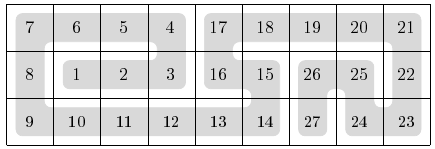
\includegraphics[]{waz.png}
	\end{center}

	뱀을 이루는 숫자들 몇개가 지워졌다. 원래 숫자를 복구하여라.
	
	\InputFile
	
	첫째 줄에는 격자판의 길이를 나타내는 정수 $n$이 주어진다. ($1 \le n \le 1,000$) 다음 세개의 줄의 $i$번째 줄은 공백 하나로 구분된 $n$개의 정수가 주어진다. $i$번째 줄의 $j$번째 숫자를 $a_{ij}$라고 할 때, $a_{ij}>0$인 경우 뱀의 번호를 나타내고 $a_{ij}=0$인 경우 뱀의 번호를 알 수 없다는 것을 의미한다. ($1 \le a_{ij} \le 3n$)
	
	\OutputFile
	
	세개의 줄을 출력해야 하고, 각 줄은 $n$개의 공백 하나로 구분된 정수여야 한다. $3n$개의 숫자는 1부터 $3n$까지의 수의 순열이여야 한다. 출력은 올바른 뱀이여야 한다. 즉, 입력 데이터와 모순되지 않아야 하고, 뱀의 조건을 만족해야 한다.
	
	올바른 뱀의 배치가 존재함을 가정해도 된다. 답이 여러개인 경우, 아무것이나 하나를 출력한다.
	
	
	\SubtaskWithCost{1}{15}
	\begin{itemize}
		\item $n \le 10$
	\end{itemize}
	
	\SubtaskWithCost{2}{25}
	\begin{itemize}
		\item $n \le 40$
	\end{itemize}
	
	
	\SubtaskWithCost{3}{30}
	\begin{itemize}
		\item $n \le 300$
	\end{itemize}
	
	\SubtaskWithCost{4}{30}
	
	추가 제한조건이 없다.
	
	\Examples
		
	\begin{example}
	\exmp{
9
0 0 5 0 17 0 0 0 21
8 0 0 3 16 0 0 25 0
0 0 0 0 0 0 0 0 23


	}{%
7 6 5 4 17 18 19 20 21
8 1 2 3 16 15 26 25 22
9 10 11 12 13 14 27 24 23
	}%
	\end{example}
	
	
	
	
	
\end{problem}

